\section{Convolutional Neural Networks}

Convolutional Neural Networks (CNNs) have been  widely applied in many problems of machine
learning and computer vision in the last years \cite{krizhevsky2012imagenet,szegedy2015going}. Moreover, a lot of techniques have been proposed to enhance the performance or ease
the training of CNNs \cite{simonyan2014very,srivastava2014dropout}.

Their popularity began in 2012, following the proposition of the AlexNet network, when it outperformed all other methods for visual classification, thus attracting great attention from the research community \cite{Krizhevsky:2012:ICD:2999134.2999257}.
In the following years, an increasing adoption was observed, mainly due to the their ability to have scalable parallel processing through Graphical Processing Units (GPUs), even in usual 
desktop computers, once they are basically implemented through matrix multiplications easily parallelizable. 

\begin{figure*}[h]
\caption{Siberian Husky X Eskimo dog}
\label{fig:husky}
  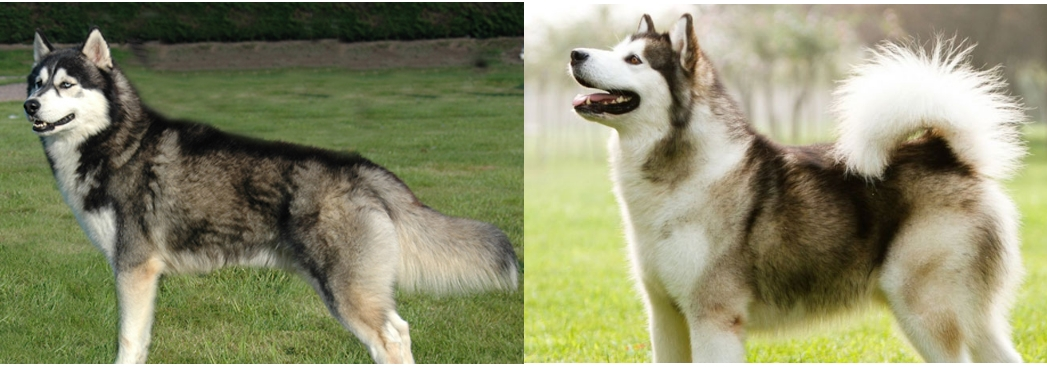
\includegraphics[width=\textwidth]{images/husky.jpg}
\end{figure*}

Studies reveal that when trained efficiently, CNNs are able
to map complex, high-dimensional image data into a much lower dimensional space of finite
distinct categories, composed of hundreds or thousands object classes. Categories may be smoothly different, as evidentiated in a possible distinction of a Siberian Husky and a Eskimo dog (Figure \ref{fig:husky}). CNNs have also been successfully employed in a vast domain of applications, such as video object detection, speech recognition and language translation \cite{liu2017survey}.

Their architecture consists basically of a stack of three types of layers, namely convolutional layers, pooling layers and fully-connected layers. A typical CNN network is depicted in Figure \ref{fig:mnist}, for the MNIST dataset digit classification. A convolutional layer determines the output of neurons associated to local regions of the input, by means of the scalar product between their weights and the region representing the input volume. The ReLu (rectified linear unit) rectifier applies an elementwise activation function (eg. sigmoid) to the output of the activation  generated by the previous layer. A pooling layer, in turn,  downlsamples along the spatial dimensionality of the input, thus reducing the quantity of parameters in the current activation. Finally, a fully-connected layer is responsible for producing class scores from activations, for classification purposes. For improving performance, ReLu is also commonly employed between these layers. 


\begin{figure*}[h]
\caption{Standard CNN architecture}
\label{fig:mnist}
  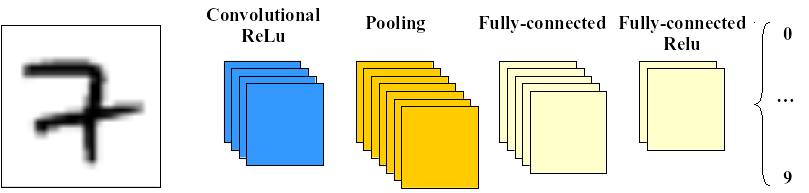
\includegraphics[width=\textwidth]{images/CNN.png}
\end{figure*}
